\documentclass[svgnames,11pt]{beamer}
\input{/home/tof/Documents/Cozy/latex-include/preambule_commun.tex}
\input{/home/tof/Documents/Cozy/latex-include/preambule_beamer.tex}
%\usepackage{pgfpages} \setbeameroption{show notes on second screen=left}
\author[]{Christophe Viroulaud}
\title{Représentation d'un graphe\\en POO}
\date{\framebox{\textbf{Algo 22}}}
%\logo{}
\institute{Terminale - NSI}

\begin{document}
\begin{frame}
\titlepage
\end{frame}
\begin{frame}
    \frametitle{}

    \begin{center}
        Les graphes sont des outils très utilisés en informatique. Il semble donc intéressant de disposer d'une bibliothèque fournissant les outils nécessaires à la création et la manipulation d'un graphe.
    \end{center}

\end{frame}
\begin{frame}
    \frametitle{}

    \begin{framed}
        \centering Construire une bibliothèque \textbf{\texttt{graphe}}.
    \end{framed}

\end{frame}
\section{Conception}
\subsection{Différents graphes}
\begin{frame}
    \frametitle{Conception - Différents graphes}

\begin{multicols}{3}    
    \begin{center}
        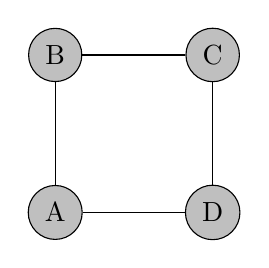
\begin{tikzpicture}
            \node[draw,circle,fill=gray!50] (A)at(0,0) {A};
            \node[draw,circle,fill=gray!50] (B)at(0,2) {B};
            \node[draw,circle,fill=gray!50] (C)at(2,2) {C};
            \node[draw,circle,fill=gray!50] (D)at(2,0) {D};


            \draw (A) -- (B);
            \draw (A) -- (D);
            \draw (B) -- (C);
            \draw (C) -- (D);

        \end{tikzpicture}
    \end{center}
    \begin{center}
        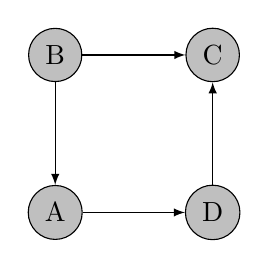
\begin{tikzpicture}
            \node[draw,circle,fill=gray!50] (A)at(0,0) {A};
            \node[draw,circle,fill=gray!50] (B)at(0,2) {B};
            \node[draw,circle,fill=gray!50] (C)at(2,2) {C};
            \node[draw,circle,fill=gray!50] (D)at(2,0) {D};


            \draw[<-,>=latex] (A) -- (B);
            \draw[->,>=latex] (A) -- (D);
            \draw[->,>=latex] (B) -- (C);
            \draw[<-,>=latex] (C) -- (D);

        \end{tikzpicture}
    \end{center}
    \begin{center}
        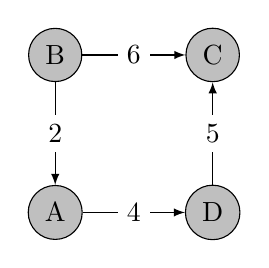
\begin{tikzpicture}
            \node[draw,circle,fill=gray!50] (A)at(0,0) {A};
            \node[draw,circle,fill=gray!50] (B)at(0,2) {B};
            \node[draw,circle,fill=gray!50] (C)at(2,2) {C};
            \node[draw,circle,fill=gray!50] (D)at(2,0) {D};


            \draw[<-,>=latex] (A) -- (B)node[midway, fill=white] {2};
            \draw[->,>=latex] (A) -- (D)node[midway, fill=white] {4};
            \draw[->,>=latex] (B) -- (C)node[midway, fill=white] {6};
            \draw[<-,>=latex] (C) -- (D)node[midway, fill=white] {5};

        \end{tikzpicture}
    \end{center}
\end{multicols}
\begin{aretenir}[Observation]
La bibliothèque \textbf{\texttt{graphe}} doit prendre en compte les différents cas de figures.
\end{aretenir}
\end{frame}
\begin{frame}
    \frametitle{}

    \begin{itemize}
        \item Une arête non-orientée est équivalente à deux arêtes orientées de sens opposé.
        \item Un graphe non pondéré est équivalent à un graphe où toutes les pondérations valent 1.
    \end{itemize}

\end{frame}
\subsection{Les ensembles}
\begin{frame}
    \frametitle{Les ensembles}
\begin{aretenir}[]
    Un ensemble est une collection non ordonnée sans éléments en double. \url{https://tinyurl.com/set-pyt}
\end{aretenir}
    

\end{frame}
\begin{frame}[fragile]
    \frametitle{}

    \begin{center}
        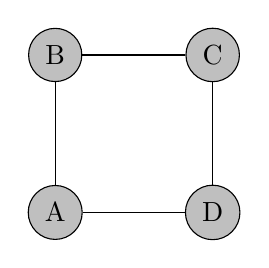
\begin{tikzpicture}
            \node[draw,circle,fill=gray!50] (A)at(0,0) {A};
            \node[draw,circle,fill=gray!50] (B)at(0,2) {B};
            \node[draw,circle,fill=gray!50] (C)at(2,2) {C};
            \node[draw,circle,fill=gray!50] (D)at(2,0) {D};


            \draw (A) -- (B);
            \draw (A) -- (D);
            \draw (B) -- (C);
            \draw (C) -- (D);

        \end{tikzpicture}
    \end{center}
    \begin{center}
    \begin{lstlisting}[language=Python , basicstyle=\ttfamily\small, xleftmargin=2em, xrightmargin=2em]
voisins_B = { ("A", 1), ("D", 1) }
\end{lstlisting}
    \captionof{code}{Ensemble des voisins de B}
    \label{CODE}
    \end{center}
\end{frame}
\begin{frame}[fragile]
    \frametitle{}

    
\begin{aretenir}[Remarque]
\begin{center}
\begin{lstlisting}[language=Python , basicstyle=\ttfamily\small, xleftmargin=2em, xrightmargin=2em]
# Crée un ensemble vide
e = set()

# Crée un dictionnaire vide
d = {}
\end{lstlisting}
\end{center}
\end{aretenir}

\end{frame}
\section{Implémentation}
\subsection{Classe \textbf{\texttt{Graphe}}}
\begin{frame}
    \frametitle{Implémentation - Classe \textbf{\texttt{Graphe}}}

\begin{activite}
\begin{enumerate}
    \item Créer le fichier \textbf{\texttt{biblio\_graphe.py}}
    \item Construire la classe \textbf{\texttt{Graphe}} et son constructeur qui initialisera:
    \begin{itemize}
        \item un attribut booléen \textbf{\texttt{oriente}} qui sera initialisé par une valeur booléenne passée en paramètre.
        \item un dictionnaire vide nommé \textbf{\texttt{sommets}}.
    \end{itemize} 
\end{enumerate}
\end{activite}

\end{frame}
\begin{frame}
    \frametitle{Avant de regarder la correction}
\begin{center}
    \centering
    \includegraphics[width=3cm]{/home/tof/Documents/Cozy/latex-include/stop.png}
    \end{center}
{\Large
    \begin{itemize}
        \item Prendre le temps de réfléchir,
        \item Analyser les messages d'erreur,
        \item Demander au professeur.
    \end{itemize}
}
\end{frame}
\begin{frame}[fragile]
    \frametitle{Correction}
\begin{center}
\begin{lstlisting}[language=Python , basicstyle=\ttfamily\small, xleftmargin=1.5em, xrightmargin=2em]
class Graphe:
    def __init__(self, oriente: bool):
        self.sommets = {}
        self.oriente = oriente
\end{lstlisting}
\end{center}
    

\end{frame}
\begin{frame}
    \frametitle{}

    \begin{activite}
    \begin{enumerate}
        
    \item Écrire la méthode \textbf{\texttt{ajouter\_sommet(self, s: str) $\rightarrow$ None}} qui ajoute un nouveau sommet dans le dictionnaire \textbf{\texttt{sommets}} s'il n'est pas déjà présent. Un ensemble vide sera associé au sommet.
    \item Écrire la méthode \textbf{\texttt{ajouter\_arete(self, s1: str, s2: str, d: int = 1) $\rightarrow$ None}} qui crée une arête, éventuellement orientée de \textbf{\texttt{s1}} vers \textbf{\texttt{s2}}, de pondération \textbf{\texttt{d}}. Si la pondération n'est pas précisée la valeur \textbf{\texttt{1}} est utilisée par défaut. Si les sommets n'existent pas, la méthode devra les créer préalablement.
    \end{enumerate}
    \end{activite}

\end{frame}
\begin{frame}
    \frametitle{Avant de regarder la correction}
\begin{center}
    \centering
    \includegraphics[width=3cm]{/home/tof/Documents/Cozy/latex-include/stop.png}
    \end{center}
{\Large
    \begin{itemize}
        \item Prendre le temps de réfléchir,
        \item Analyser les messages d'erreur,
        \item Demander au professeur.
    \end{itemize}
}
\end{frame}
\begin{frame}[fragile]
    \frametitle{Correction}

\begin{center}
\begin{lstlisting}[language=Python , basicstyle=\ttfamily\small, xleftmargin=2em, xrightmargin=2em]
def ajouter_sommet(self, s: str) -> None:
    if not(s in self.sommets):
        self.sommets[s] = set()

def ajouter_arete(self, s1: str, s2: str, d: int = 1) -> None:
    # ajout éventuel des sommets
    self.ajouter_sommet(s1)
    self.ajouter_sommet(s2)
    # création arête
    self.sommets[s1].add((s2, d))
    if not self.oriente:
        self.sommets[s2].add((s1, d))
\end{lstlisting}
\end{center}

\end{frame}
\begin{frame}
    \frametitle{}
    \begin{center}
        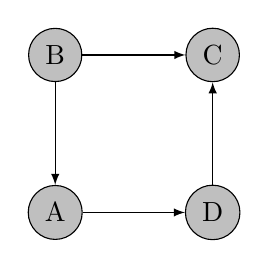
\begin{tikzpicture}
            \node[draw,circle,fill=gray!50] (A)at(0,0) {A};
            \node[draw,circle,fill=gray!50] (B)at(0,2) {B};
            \node[draw,circle,fill=gray!50] (C)at(2,2) {C};
            \node[draw,circle,fill=gray!50] (D)at(2,0) {D};


            \draw[<-,>=latex] (A) -- (B);
            \draw[->,>=latex] (A) -- (D);
            \draw[->,>=latex] (B) -- (C);
            \draw[<-,>=latex] (C) -- (D);

        \end{tikzpicture}
        \captionof{figure}{Exemple}
        \label{exemple}
    \end{center}
    \begin{activite}
    \begin{enumerate}
        \item Créer un fichier \textbf{\texttt{exemple.py}}
        \item Importer la bibliothèque et créer une instance de \textbf{\texttt{Graphe}} représentant le graphe (figure \ref{exemple}).
        \item Dans la classe \textbf{\texttt{Graphe}} créer la méthode \textbf{\texttt{affiche\_voisins(self, s: str) $\rightarrow$ None}} qui affiche dans la console les voisins de \textbf{\texttt{s}} ainsi que la distance entre les 2 sommets. 
    \end{enumerate}
    \end{activite}

\end{frame}
\begin{frame}
    \frametitle{Avant de regarder la correction}
\begin{center}
    \centering
    \includegraphics[width=3cm]{/home/tof/Documents/Cozy/latex-include/stop.png}
    \end{center}
{\Large
    \begin{itemize}
        \item Prendre le temps de réfléchir,
        \item Analyser les messages d'erreur,
        \item Demander au professeur.
    \end{itemize}
}
\end{frame}
\begin{frame}[fragile]
    \frametitle{Correction}

\begin{center}
\begin{lstlisting}[language=Python , basicstyle=\ttfamily\small, xleftmargin=2em, xrightmargin=2em]
exemple = Graphe()
exemple.ajouter_arete("A", "D")
exemple.ajouter_arete("D", "C")
exemple.ajouter_arete("B", "A")
exemple.ajouter_arete("B", "C")
\end{lstlisting}
\captionof{code}{Instanciation}
\label{CODE}
\end{center}

\end{frame}
\begin{frame}[fragile]
    \frametitle{}

\begin{center}
\begin{lstlisting}[language=Python , basicstyle=\ttfamily\small, xleftmargin=2em, xrightmargin=2em]
def affiche_voisins(self, s: str) -> None:
    for v in self.sommets[s]:
        print(f"{s} --> {v[0]} : {v[1]}")
\end{lstlisting}
\captionof{code}{Méthode d'affichage}
\begin{lstlisting}[language=Python , basicstyle=\ttfamily\small, xleftmargin=2em, xrightmargin=2em]
>>> exemple.affiche_voisins("B")
B --> A : 1
B --> C : 1
\end{lstlisting}
    \captionof{code}{Appel de la méthode}
\end{center}

\end{frame}
\subsection{Méthodes de parcours}
\begin{frame}
    \frametitle{Méthodes de parcours}
\begin{activite}
\begin{enumerate}
    \item Dans le même dossier que la bibliothèque, placer le fichier \textbf{\texttt{structures.py}} construit dans les cours précédents.
    \item Écrire la méthode itérative \textbf{\texttt{dfs\_it(self, s: str) $\rightarrow$ list}} qui renvoie la liste des sommets visités depuis \textbf{\texttt{s}} avec un parcours en profondeur.
    \item \textbf{Pour les plus avancés:} Écrire la méthode récursive \textbf{\texttt{dfs\_rec(self, s: str, parcours: list)} $\rightarrow$ list}.
\end{enumerate}
\end{activite}
    
\end{frame}
\begin{frame}
    \frametitle{Avant de regarder la correction}
\begin{center}
    \centering
    \includegraphics[width=3cm]{/home/tof/Documents/Cozy/latex-include/stop.png}
    \end{center}
{\Large
    \begin{itemize}
        \item Prendre le temps de réfléchir,
        \item Analyser les messages d'erreur,
        \item Demander au professeur.
    \end{itemize}
}
\end{frame}
\begin{frame}[fragile]
    \frametitle{Correction}

\begin{center}
\begin{lstlisting}[language=Python , basicstyle=\ttfamily\small, xleftmargin=0.2em, xrightmargin=0em]
def dfs_it(self, s: str) -> list:
    parcours = []
    p = Pile()
    p.empiler(s)
    while not p.est_vide():
        en_cours = p.depiler()
        if en_cours not in parcours:
            parcours.append(en_cours)
            
            for voisin in self.sommets[en_cours]:
                p.empiler(voisin[0])
                
    return parcours
\end{lstlisting}
\begin{lstlisting}[language=Python , basicstyle=\ttfamily\small, xleftmargin=0.2em, xrightmargin=0em]
>>> exemple.dfs_it("A")
['A', 'D', 'C']
\end{lstlisting}
\end{center}  

\end{frame}
\begin{frame}[fragile]
    \frametitle{}

\begin{center}
\begin{lstlisting}[language=Python , basicstyle=\ttfamily\small, xleftmargin=0.2em, xrightmargin=0em]
def dfs_rec(self, s: str, parcours: list) -> None:
    """
    version récursive du parcours en profondeur

    Args:
        s (str): départ
        parcours (list): sommets traversés
    """
    if s not in parcours:
        parcours.append(s)
        for voisin in self.sommets[s]:
            self.dfs_rec(voisin[0], parcours)
\end{lstlisting}
\begin{lstlisting}[language=Python , basicstyle=\ttfamily\small, xleftmargin=0.2em, xrightmargin=0em]
>>> parcours_rec = []
>>> exemple.dfs_rec("A", parcours_rec)
>>> parcours_rec
['A', 'D', 'C'] 
\end{lstlisting}
\end{center} 

\end{frame}
\section{Application}
\begin{frame}
    \frametitle{Application}

    \begin{center}
        \centering
        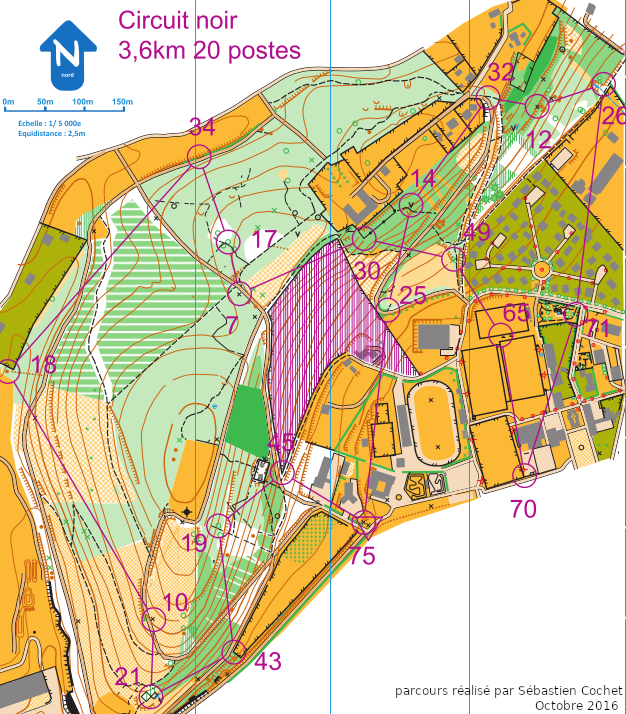
\includegraphics[width=7cm]{ressources/co-noir.png}
    \end{center}

\end{frame}
\begin{frame}

    \begin{center}
        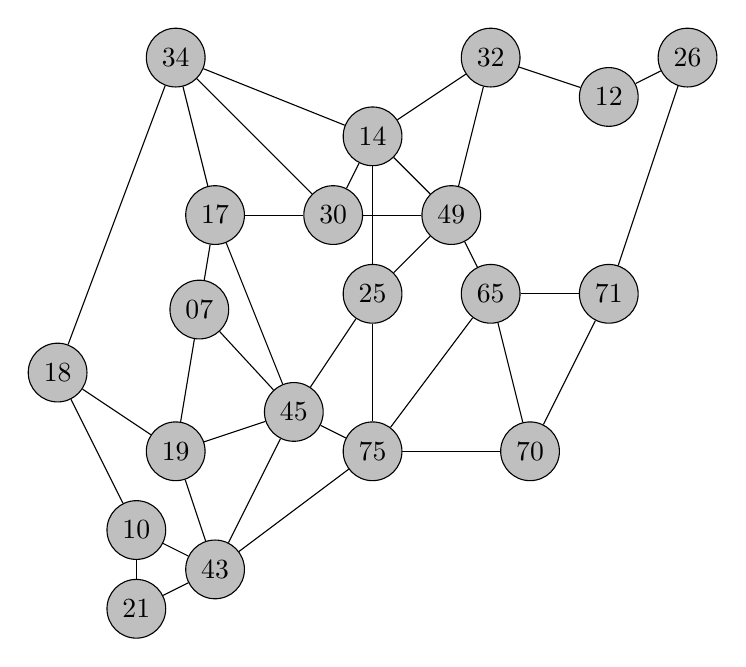
\begin{tikzpicture}
            \node[draw,circle,fill=gray!50] (21)at(0,0) {21};
            \node[draw,circle,fill=gray!50] (43)at(1,0.5) {43};
            \node[draw,circle,fill=gray!50] (10)at(0,1) {10};
            \node[draw,circle,fill=gray!50] (19)at(0.5,2) {19};
            \node[draw,circle,fill=gray!50] (45)at(2,2.5) {45};
            \node[draw,circle,fill=gray!50] (18)at(-1,3) {18};
            \node[draw,circle,fill=gray!50] (75)at(3,2) {75};
            \node[draw,circle,fill=gray!50] (70)at(5,2) {70};
            \node[draw,circle,fill=gray!50] (65)at(4.5,4) {65};
            \node[draw,circle,fill=gray!50] (71)at(6,4) {71};
            \node[draw,circle,fill=gray!50] (25)at(3,4) {25};
            \node[draw,circle,fill=gray!50] (07)at(0.8,3.8) {07};
            \node[draw,circle,fill=gray!50] (17)at(1,5) {17};
            \node[draw,circle,fill=gray!50] (30)at(2.5,5) {30};
            \node[draw,circle,fill=gray!50] (49)at(4,5) {49};
            \node[draw,circle,fill=gray!50] (14)at(3,6) {14};
            \node[draw,circle,fill=gray!50] (34)at(0.5,7) {34};
            \node[draw,circle,fill=gray!50] (32)at(4.5,7) {32};
            \node[draw,circle,fill=gray!50] (12)at(6,6.5) {12};
            \node[draw,circle,fill=gray!50] (26)at(7,7) {26};

            \draw[-,>=latex] (75) -- (45);
            \draw[-,>=latex] (75) -- (25);
            \draw[-,>=latex] (75) -- (65);
            \draw[-,>=latex] (75) -- (70);
            \draw[-,>=latex] (75) -- (43);
            \draw[-,>=latex] (45) -- (07);
            \draw[-,>=latex] (45) -- (43);
            \draw[-,>=latex] (45) -- (25);
            \draw[-,>=latex] (45) -- (19);
            \draw[-,>=latex] (45) -- (17);
            \draw[-,>=latex] (25) -- (14);
            %\draw[-,>=latex] (19) -- (10);
            \draw[-,>=latex] (19) -- (18);
            \draw[-,>=latex] (19) -- (07);
            \draw[-,>=latex] (19) -- (43);
            \draw[-,>=latex] (43) -- (10);
            \draw[-,>=latex] (43) -- (21);
            %\draw[-,>=latex] (43) -- (18);
            \draw[-,>=latex] (10) -- (21);
            \draw[-,>=latex] (10) -- (18);
            \draw[-,>=latex] (34) -- (17);
            \draw[-,>=latex] (70) -- (71);
            \draw[-,>=latex] (70) -- (65);
            \draw[-,>=latex] (49) -- (65);
            \draw[-,>=latex] (49) -- (25);
            \draw[-,>=latex] (49) -- (14);
            \draw[-,>=latex] (49) -- (30);
            \draw[-,>=latex] (49) -- (32);
            \draw[-,>=latex] (30) -- (14);
            \draw[-,>=latex] (30) -- (34);
            \draw[-,>=latex] (30) -- (17);
            \draw[-,>=latex] (14) -- (34);
            \draw[-,>=latex] (14) -- (32);
            \draw[-,>=latex] (32) -- (12);
            \draw[-,>=latex] (12) -- (26);
            \draw[-,>=latex] (65) -- (71);
            \draw[-,>=latex] (71) -- (26);
            \draw[-,>=latex] (18) -- (34);
            \draw[-,>=latex] (07) -- (17);

        \end{tikzpicture}
        \captionof{figure}{Graphe représentatif de la carte de CO}
    \end{center}

    

\end{frame}
\begin{frame}
    \frametitle{}

    \begin{activite}
    \begin{enumerate}
        \item Placer le fichier \textbf{\texttt{parcours\_noir.json}} dans le même dossier que la bibliothèque.
        \item Créer un fichier \textbf{\texttt{parcours\_co.py}}
        \item Construire une instance de \textbf{\texttt{Graphe}} représentative de la carte de CO.
    \end{enumerate}
    \end{activite}

\end{frame}
\begin{frame}
    \frametitle{Avant de regarder la correction}
\begin{center}
    \centering
    \includegraphics[width=3cm]{/home/tof/Documents/Cozy/latex-include/stop.png}
    \end{center}
{\Large
    \begin{itemize}
        \item Prendre le temps de réfléchir,
        \item Analyser les messages d'erreur,
        \item Demander au professeur.
    \end{itemize}
}
\end{frame}
\begin{frame}[fragile]
    \frametitle{Correction}
\begin{center}
\begin{lstlisting}[language=Python , basicstyle=\ttfamily\small, xleftmargin=0.2em, xrightmargin=0em]
import json
from biblio_graphe import Graphe

# chargement du json
f = open("parcours_noir.json")
list_graphe = json.load(f)

graphe = Graphe(False)
# parcours du graphe
for couple in list_graphe:
    sommet = couple["sommet"]
    adjacents = couple["adjacents"]
    for voisin in adjacents:
        # les sommets sont ajoutés automatiquement
        graphe.ajouter_arete(sommet, voisin)
        
f.close()
\end{lstlisting}
\end{center}
    

\end{frame}
\section{Pour aller plus loin}
\begin{frame}
    \frametitle{Pour aller plus loin}

    Considérons un graphe non orienté et non pondéré. Un parcours en largeur permet de déterminer le plus court chemin entre deux sommets. En effet, le parcours \emph{s'éloigne} de l'origine niveau après niveau. Il suffit alors de maintenir un dictionnaire des sommets visités associés à leur prédécesseur pour retrouver le chemin le plus court partant de l'origine jusqu'à n'importe quel sommet.

\end{frame}

\begin{frame}

    \begin{center}
        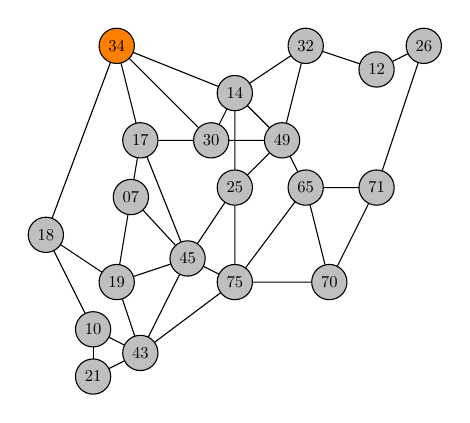
\begin{tikzpicture}[scale=0.6, transform shape]
            \node[draw,circle,fill=gray!50] (21)at(0,0) {21};
            \node[draw,circle,fill=gray!50] (43)at(1,0.5) {43};
            \node[draw,circle,fill=gray!50] (10)at(0,1) {10};
            \node[draw,circle,fill=gray!50] (19)at(0.5,2) {19};
            \node[draw,circle,fill=gray!50] (45)at(2,2.5) {45};
            \node[draw,circle,fill=gray!50] (18)at(-1,3) {18};
            \node[draw,circle,fill=gray!50] (75)at(3,2) {75};
            \node[draw,circle,fill=gray!50] (70)at(5,2) {70};
            \node[draw,circle,fill=gray!50] (65)at(4.5,4) {65};
            \node[draw,circle,fill=gray!50] (71)at(6,4) {71};
            \node[draw,circle,fill=gray!50] (25)at(3,4) {25};
            \node[draw,circle,fill=gray!50] (07)at(0.8,3.8) {07};
            \node[draw,circle,fill=gray!50] (17)at(1,5) {17};
            \node[draw,circle,fill=gray!50] (30)at(2.5,5) {30};
            \node[draw,circle,fill=gray!50] (49)at(4,5) {49};
            \node[draw,circle,fill=gray!50] (14)at(3,6) {14};
            \node[draw,circle,fill=orange] (34)at(0.5,7) {34};
            \node[draw,circle,fill=gray!50] (32)at(4.5,7) {32};
            \node[draw,circle,fill=gray!50] (12)at(6,6.5) {12};
            \node[draw,circle,fill=gray!50] (26)at(7,7) {26};

            \draw[-,>=latex] (75) -- (45);
            \draw[-,>=latex] (75) -- (25);
            \draw[-,>=latex] (75) -- (65);
            \draw[-,>=latex] (75) -- (70);
            \draw[-,>=latex] (75) -- (43);
            \draw[-,>=latex] (45) -- (07);
            \draw[-,>=latex] (45) -- (43);
            \draw[-,>=latex] (45) -- (25);
            \draw[-,>=latex] (45) -- (19);
            \draw[-,>=latex] (45) -- (17);
            \draw[-,>=latex] (25) -- (14);
            %\draw[-,>=latex] (19) -- (10);
            \draw[-,>=latex] (19) -- (18);
            \draw[-,>=latex] (19) -- (07);
            \draw[-,>=latex] (19) -- (43);
            \draw[-,>=latex] (43) -- (10);
            \draw[-,>=latex] (43) -- (21);
            %\draw[-,>=latex] (43) -- (18);
            \draw[-,>=latex] (10) -- (21);
            \draw[-,>=latex] (10) -- (18);
            \draw[-,>=latex] (34) -- (17);
            \draw[-,>=latex] (70) -- (71);
            \draw[-,>=latex] (70) -- (65);
            \draw[-,>=latex] (49) -- (65);
            \draw[-,>=latex] (49) -- (25);
            \draw[-,>=latex] (49) -- (14);
            \draw[-,>=latex] (49) -- (30);
            \draw[-,>=latex] (49) -- (32);
            \draw[-,>=latex] (30) -- (14);
            \draw[-,>=latex] (30) -- (34);
            \draw[-,>=latex] (30) -- (17);
            \draw[-,>=latex] (14) -- (34);
            \draw[-,>=latex] (14) -- (32);
            \draw[-,>=latex] (32) -- (12);
            \draw[-,>=latex] (12) -- (26);
            \draw[-,>=latex] (65) -- (71);
            \draw[-,>=latex] (71) -- (26);
            \draw[-,>=latex] (18) -- (34);
            \draw[-,>=latex] (07) -- (17);

        \end{tikzpicture}
        \captionof{figure}{Plus court chemin entre 34 et 19.}
    \end{center}

    \begin{itemize}
        \item 34: niveau 0
    \end{itemize}

\end{frame}

\begin{frame}

    \begin{center}
        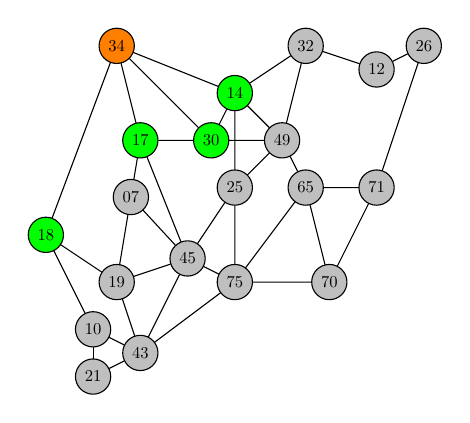
\begin{tikzpicture}[scale=0.6, transform shape]
            \node[draw,circle,fill=gray!50] (21)at(0,0) {21};
            \node[draw,circle,fill=gray!50] (43)at(1,0.5) {43};
            \node[draw,circle,fill=gray!50] (10)at(0,1) {10};
            \node[draw,circle,fill=gray!50] (19)at(0.5,2) {19};
            \node[draw,circle,fill=gray!50] (45)at(2,2.5) {45};
            \node[draw,circle,fill=green] (18)at(-1,3) {18};
            \node[draw,circle,fill=gray!50] (75)at(3,2) {75};
            \node[draw,circle,fill=gray!50] (70)at(5,2) {70};
            \node[draw,circle,fill=gray!50] (65)at(4.5,4) {65};
            \node[draw,circle,fill=gray!50] (71)at(6,4) {71};
            \node[draw,circle,fill=gray!50] (25)at(3,4) {25};
            \node[draw,circle,fill=gray!50] (07)at(0.8,3.8) {07};
            \node[draw,circle,fill=green] (17)at(1,5) {17};
            \node[draw,circle,fill=green] (30)at(2.5,5) {30};
            \node[draw,circle,fill=gray!50] (49)at(4,5) {49};
            \node[draw,circle,fill=green] (14)at(3,6) {14};
            \node[draw,circle,fill=orange] (34)at(0.5,7) {34};
            \node[draw,circle,fill=gray!50] (32)at(4.5,7) {32};
            \node[draw,circle,fill=gray!50] (12)at(6,6.5) {12};
            \node[draw,circle,fill=gray!50] (26)at(7,7) {26};

            \draw[-,>=latex] (75) -- (45);
            \draw[-,>=latex] (75) -- (25);
            \draw[-,>=latex] (75) -- (65);
            \draw[-,>=latex] (75) -- (70);
            \draw[-,>=latex] (75) -- (43);
            \draw[-,>=latex] (45) -- (07);
            \draw[-,>=latex] (45) -- (43);
            \draw[-,>=latex] (45) -- (25);
            \draw[-,>=latex] (45) -- (19);
            \draw[-,>=latex] (45) -- (17);
            \draw[-,>=latex] (25) -- (14);
            %\draw[-,>=latex] (19) -- (10);
            \draw[-,>=latex] (19) -- (18);
            \draw[-,>=latex] (19) -- (07);
            \draw[-,>=latex] (19) -- (43);
            \draw[-,>=latex] (43) -- (10);
            \draw[-,>=latex] (43) -- (21);
            %\draw[-,>=latex] (43) -- (18);
            \draw[-,>=latex] (10) -- (21);
            \draw[-,>=latex] (10) -- (18);
            \draw[-,>=latex] (34) -- (17);
            \draw[-,>=latex] (70) -- (71);
            \draw[-,>=latex] (70) -- (65);
            \draw[-,>=latex] (49) -- (65);
            \draw[-,>=latex] (49) -- (25);
            \draw[-,>=latex] (49) -- (14);
            \draw[-,>=latex] (49) -- (30);
            \draw[-,>=latex] (49) -- (32);
            \draw[-,>=latex] (30) -- (14);
            \draw[-,>=latex] (30) -- (34);
            \draw[-,>=latex] (30) -- (17);
            \draw[-,>=latex] (14) -- (34);
            \draw[-,>=latex] (14) -- (32);
            \draw[-,>=latex] (32) -- (12);
            \draw[-,>=latex] (12) -- (26);
            \draw[-,>=latex] (65) -- (71);
            \draw[-,>=latex] (71) -- (26);
            \draw[-,>=latex] (18) -- (34);
            \draw[-,>=latex] (07) -- (17);

        \end{tikzpicture}
        \captionof{figure}{Plus court chemin entre 34 et 19.}
    \end{center}

    \begin{itemize}
        \item 34: niveau 0
        \item 14 - 30 - 17 - 18: niveau 1
    \end{itemize}

\end{frame}
\begin{frame}

    \begin{center}
        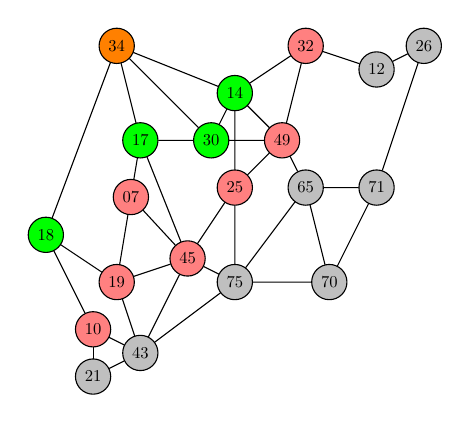
\begin{tikzpicture}[scale=0.6, transform shape]
            \node[draw,circle,fill=gray!50] (21)at(0,0) {21};
            \node[draw,circle,fill=gray!50] (43)at(1,0.5) {43};
            \node[draw,circle,fill=red!50] (10)at(0,1) {10};
            \node[draw,circle,fill=red!50] (19)at(0.5,2) {19};
            \node[draw,circle,fill=red!50] (45)at(2,2.5) {45};
            \node[draw,circle,fill=green] (18)at(-1,3) {18};
            \node[draw,circle,fill=gray!50] (75)at(3,2) {75};
            \node[draw,circle,fill=gray!50] (70)at(5,2) {70};
            \node[draw,circle,fill=gray!50] (65)at(4.5,4) {65};
            \node[draw,circle,fill=gray!50] (71)at(6,4) {71};
            \node[draw,circle,fill=red!50] (25)at(3,4) {25};
            \node[draw,circle,fill=red!50] (07)at(0.8,3.8) {07};
            \node[draw,circle,fill=green] (17)at(1,5) {17};
            \node[draw,circle,fill=green] (30)at(2.5,5) {30};
            \node[draw,circle,fill=red!50] (49)at(4,5) {49};
            \node[draw,circle,fill=green] (14)at(3,6) {14};
            \node[draw,circle,fill=orange] (34)at(0.5,7) {34};
            \node[draw,circle,fill=red!50] (32)at(4.5,7) {32};
            \node[draw,circle,fill=gray!50] (12)at(6,6.5) {12};
            \node[draw,circle,fill=gray!50] (26)at(7,7) {26};

            \draw[-,>=latex] (75) -- (45);
            \draw[-,>=latex] (75) -- (25);
            \draw[-,>=latex] (75) -- (65);
            \draw[-,>=latex] (75) -- (70);
            \draw[-,>=latex] (75) -- (43);
            \draw[-,>=latex] (45) -- (07);
            \draw[-,>=latex] (45) -- (43);
            \draw[-,>=latex] (45) -- (25);
            \draw[-,>=latex] (45) -- (19);
            \draw[-,>=latex] (45) -- (17);
            \draw[-,>=latex] (25) -- (14);
            %\draw[-,>=latex] (19) -- (10);
            \draw[-,>=latex] (19) -- (18);
            \draw[-,>=latex] (19) -- (07);
            \draw[-,>=latex] (19) -- (43);
            \draw[-,>=latex] (43) -- (10);
            \draw[-,>=latex] (43) -- (21);
            %\draw[-,>=latex] (43) -- (18);
            \draw[-,>=latex] (10) -- (21);
            \draw[-,>=latex] (10) -- (18);
            \draw[-,>=latex] (34) -- (17);
            \draw[-,>=latex] (70) -- (71);
            \draw[-,>=latex] (70) -- (65);
            \draw[-,>=latex] (49) -- (65);
            \draw[-,>=latex] (49) -- (25);
            \draw[-,>=latex] (49) -- (14);
            \draw[-,>=latex] (49) -- (30);
            \draw[-,>=latex] (49) -- (32);
            \draw[-,>=latex] (30) -- (14);
            \draw[-,>=latex] (30) -- (34);
            \draw[-,>=latex] (30) -- (17);
            \draw[-,>=latex] (14) -- (34);
            \draw[-,>=latex] (14) -- (32);
            \draw[-,>=latex] (32) -- (12);
            \draw[-,>=latex] (12) -- (26);
            \draw[-,>=latex] (65) -- (71);
            \draw[-,>=latex] (71) -- (26);
            \draw[-,>=latex] (18) -- (34);
            \draw[-,>=latex] (07) -- (17);

        \end{tikzpicture}
        \captionof{figure}{Plus court chemin entre 34 et 19.}
    \end{center}

    \begin{itemize}
        \item 34: niveau 0
        \item 14 - 30 - 17 - 18: niveau 1
        \item 32 - 49 - 25 - 45 - 07 - 19 - 10: niveau 2
    \end{itemize}

\end{frame}
\end{document}